\documentclass[12pt]{article}
\usepackage[utf8]{inputenc}
\usepackage{graphicx} % Allows you to insert figures
\usepackage{amsmath} % Allows you to do equations
\usepackage{fancyhdr} % Formats the header
\usepackage{geometry} % Formats the paper size, orientation, and margins
\usepackage{xcolor}
\usepackage{listings}
\usepackage{hyperref}
\hypersetup{
    colorlinks=true,
    linkcolor=blue,
    filecolor=magenta,      
    urlcolor=cyan,
    pdftitle={Overleaf Example},
    pdfpagemode=FullScreen,
    }
\definecolor{mGreen}{rgb}{0,0.6,0}
\definecolor{mGray}{rgb}{0.5,0.5,0.5}
\definecolor{mPurple}{rgb}{0.58,0,0.82}
\definecolor{backgroundColour}{rgb}{0.95,0.95,0.92}

\lstdefinestyle{CStyle}{
    backgroundcolor=\color{backgroundColour},   
    commentstyle=\color{mGreen},
    keywordstyle=\color{magenta},
    numberstyle=\tiny\color{mGray},
    stringstyle=\color{mPurple},
    basicstyle=\footnotesize,
    breakatwhitespace=false,         
    breaklines=true,                 
    captionpos=b,                    
    keepspaces=true,                 
    numbers=left,                    
    numbersep=5pt,                  
    showspaces=false,                
    showstringspaces=false,
    showtabs=false,                  
    tabsize=2,
    language=C
}


\usepackage[format=plain,
            labelfont=it,
            textfont=it]{caption}
\linespread{1.25} % about 1.5 spacing in Word
\setlength{\parindent}{0pt} % no paragraph indents
\setlength{\parskip}{1em} % paragraphs separated by one line
\renewcommand{\headrulewidth}{0pt}
\geometry{letterpaper, portrait, margin=1in}
\setlength{\headheight}{14.49998pt}

\newcommand\titleofdoc{Title of Document} %%%%% Put your document title in this argument
\newcommand\GroupName{Group Name} %%%%% Put your group name here. If you are the only member of the group, just put your name

\begin{document}
\begin{titlepage}
   \begin{center}
        \vspace*{4cm} % Adjust spacings to ensure the title page is generally filled with text

        \Huge{\textbf {Project Report}} 

        \vspace{0.5cm}
        \LARGE{Instructor: Dr. Avinash Eranki}
            
        \vspace{3 cm}
        \Large{Embedded Systems}
       
        \vspace{0.25cm}
        \large{Samar Singhai, Vidya Ajay, Ramanathan Annamalai}
       
        \vspace{3 cm}
        \Large{April 25, 2022}
        
        \vspace{0.25 cm}
        \Large{BM2003}
       

       \vfill
    \end{center}
\end{titlepage}

\setcounter{page}{2}
\pagestyle{fancy}
\fancyhf{}
\rhead{\thepage}
\lhead{BM2003 report}
\section*{Part 1}
\subsection*{Measuring flow rate using YFS401 and Arduino}
\subsubsection*{The YF-S401 sensor}
The YF-S401 water flow sensor consists of a PVC body, a water rotor and a hall effect sensor. When water flows through the rotor, it rolls, and its speed changes with the rate of flow. The hall effect sensor outputs the corresponding pulse signal, and this can be read using software. The sensor consists of a PVC body, and is suitable to detect flow in water dispensers, water heaters, gardening or coffee machines.

Specifications:
\begin{itemize}
    \item Max Supply Voltage: 5-12V DC
    \item Water Flow Range: 0.3-6 L/min
    \item The Output Pulse High Level: $>4.5$ VDC (DC input voltage 5 V)
    \item The Output Pulse Low Level: $<0.5$ VDC (DC input voltage 5 V)
    \item Operating Current: 15 mA (DC 5V)
\end{itemize}

\begin{figure}[h!]
    \centering
    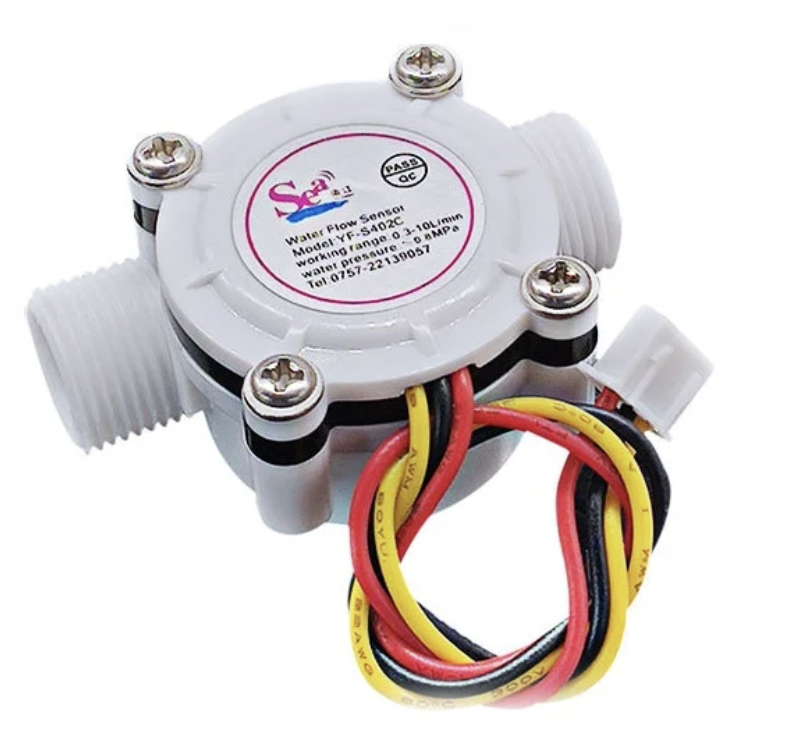
\includegraphics[scale=0.4]{sensor.png}
    \caption{The YFS401}
    \label{fig:notmy_label}
\end{figure}
\subsubsection*{The Hall-effect principle}
The effect of generating a measurable voltage in a conducting material using a magnetic field is called the Hall Effect. The basic physical principle underlying this effect is the Lorentz force
Hall Effect Sensors consist basically of a thin piece of rectangular p-type semiconductor material passing a continuous current through itself.

When the device is placed within a magnetic field, the magnetic flux lines exert a force on the semiconductor material which deflects the charge carriers, electrons and holes, to either side of the semiconductor slab. This movement of charge carriers is a result of the magnetic force they experience passing through the semiconductor material.

As these electrons and holes move sideways, a potential difference is produced between the two sides of the semiconductor material by the build-up of these charge carriers.


\subsubsection*{Calculating the water flow}
With each revolution of the wheel, the volume of fluid flowing through it is certain. At the same time, the number of pulses generated per revolution of the wheel is also a certain amount. Thus, we can establish an equation between the number of pulses and the water flow.

In fact, the YF series uses a ring magnet with six alternating poles, so that for every revolution, three low levels and three high levels, i.e., three pulses, are generated.

In the YF-S401, for every liter of water that flows, the Hall Sensor outputs  a fixed number of pulses, say "m". 

Also, the total volume of fluid flowing through the water flow sensor is equal to the water flow rate(Q - unit L/s) multiplied by time t(sec).

  Number of pulses in 1L = m\\
  So for each pulse, $\frac{1}{m}$ liters of water flows.\\
  Number of pulses in t sec = N\\
  So N pulses corresponds to $\frac{N}{m}$ liters.\\
  

\begin{gather*}
     \frac{N}{m} = V_t \\
      flow rate, Q(L/sec) = \frac{V_t}{time} \\
      Q(L/s)=\frac{N}{m*t}
\end{gather*}

\subsubsection*{Calibrating the sensor}
On using the 5880 factor (taken from the datasheet as the number of pulses in 1L), we noticed substantial errors in our water flow measurement, so we tweaked the factor around till we got an accurate reading.
The calibration factor that got us the correct reading was $\frac{5880}{4330} = 1.357$, meaning our sensor gave 4330 pulses per litre.
\subsubsection*{The Arduino code}
\begin{lstlisting}[style=Cstyle]

int inputPin=2;//input from flowmeter sensor
float flowRate;

// factor = pulses generated for 1 liter of water flow;
float factor=4330;
float volume;
float currentTime;
volatile unsigned long pulseCounter=0; //varible for counting pulses generated due to water flow

void setup() {
  Serial.begin(9600);

  //configuring pin for INPUT
  pinMode(inputPin,INPUT);
  //Initially set the inputPin to HIGH 
  digitalWrite(inputPin,HIGH);

  //for continuously checking if any Rising edge came or not, if there is rising edge call IRS_Counter() function
  attachInterrupt(digitalPinToInterrupt(inputPin),IRS_Counter,RISING);

  //millis() gives the time since arduino started, setting current time to millis()
  currentTime=millis();
  volume=0; // initial volume is zero
 
}

void loop() {

  //do all the calculations every 1 second
  if(millis()-currentTime>=1000){
    //stop checking for rising edge through interrupt
    detachInterrupt(digitalPinToInterrupt(inputPin));
    currentTime=millis(); 
    
    
    //changing the current time to millis() so millis()-currentTime=0
    // flowrate= (pulse count)/(pulses per liter) (in liter/s)
    // for milliliter/min flowrate=(pulse count)*60*1000/(pulse per liter)
    
    
    flowRate=(pulseCounter*60*1000)/factor;

    //volume=(prev volume)+(flowrate*time)
    volume+=(flowRate/60);
    
    // Serial.print("Pulse Count:");
    // Serial.println(pulseCounter);

    // printing the flowrate and volume
    Serial.print("Flow rate of water(in mL/min):");
    Serial.println(flowRate,DEC);
    Serial.print("Volume of water(mL):");
    Serial.println(volume,DEC);

    //setting pulse count to zero for another loop
      pulseCounter=0;

   // again set up the interrupt to check for rising edge
   attachInterrupt(digitalPinToInterrupt(inputPin),IRS_Counter,RISING);
  }
}

void IRS_Counter(){
  // if we hit a rising edge increase the pulse count by 1
  pulseCounter++;
}
\end{lstlisting}


\subsubsection*{The circuit setup}
\begin{figure}[h!]
\centering
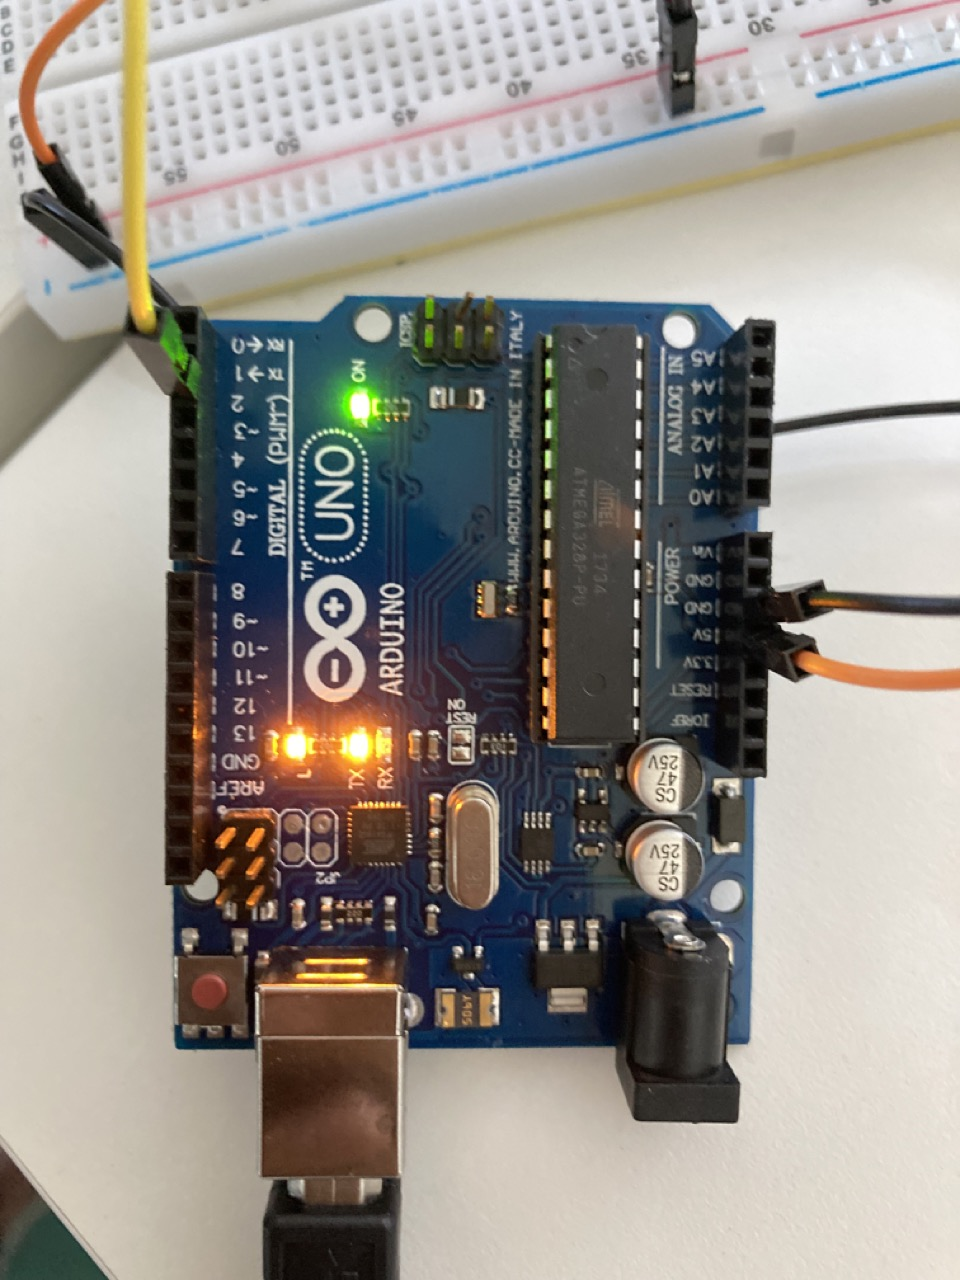
\includegraphics[scale=0.2, angle =90]{flowrate-ard.jpeg}
\caption{Arduino board connections}
\label{fig:awesome_image}
\end{figure}
\begin{figure}[h!]
\begin{minipage}{.5\textwidth}
\centering
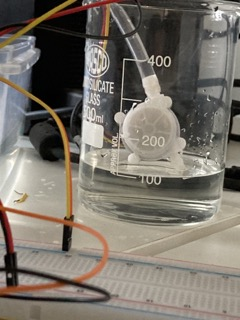
\includegraphics[scale=0.5]{water beaker.jpeg}
\caption{Water level measurement}
\label{fig:awesome_image2}
\end{minipage}%
\begin{minipage}{.5\textwidth}
\centering
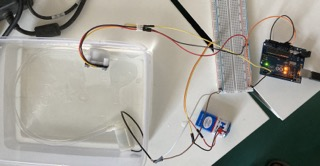
\includegraphics[scale=0.6]{water circuit.jpeg}
\caption{The measurement setup}
\label{fig:awesome_image3}
\end{minipage}
\end{figure}

\section*{Part 2}
\subsection*{Measuring water level using HC-SR04 and Arduino}
\subsubsection*{The HC-SR04 sensor}
The HC-SR04 is an ultrasonic sensor which uses sonar to calculate the distance between the sensor and the nearest object in front of it.  It is a setup of a piezoelectric sheet. Triggering the device will activate the piezoelectric sheet by creating an electric field. This generates an ultrasound. 

It has a transmitter module and a receiver module. When power is supplied to it, the transmitter module emits a sound wave which is reflected at the nearest surface. This wave travels back to the receiver, and the time elapsed is recorded. This sensor can detect surfaces up to 4 meters away from it. 

On working the sensor with Arduino, we observed a high pulse signal as the output from the device every time a surface was introduced close to it.

\begin{figure}[h!]
    \centering
    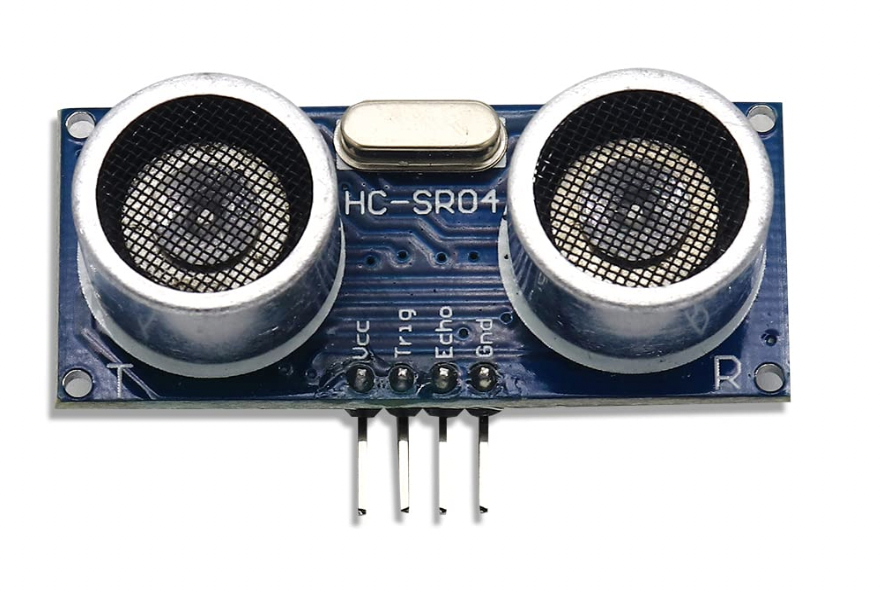
\includegraphics[scale=0.4]{hcsr04.png}
    \caption{The HC-SR04}
    \label{fig:my_label}
\end{figure}
The sensor has four pins:\begin{itemize}

    \item Pin1 ($V_{cc}$): This pin provides a +5V power supply to the sensor.
    \item Pin2 (Trigger): This is an input pin, and it initializes measurement by transmitting ultrasonic waves, on keeping this pin high for 10µs.
    \item Pin3 (Echo): This is an output pin, which gives a high signal until the wave returns back to the sensor.
    \item Pin4 (GND): This is a ground pin.
\end{itemize}

Specifications:
\begin{itemize}

    \item Operating Voltage:  5V DC
    \item Operating Current:  15mA
    \item Max Range:	4m
    \item Min Range:	2cm
    \item Ranging Accuracy:	3mm
     \item Operating Frequency:	40KHz
\end{itemize}


\subsubsection*{Calculating distance}

When a pulse of at least 10 µS (10 microseconds) in duration is applied to the Trigger pin, the sensor transmits a sonic burst of eight pulses at 40 KHz. This 8-pulse pattern makes the “ultrasonic signature” from the device unique, allowing the receiver to differentiate the transmitted pattern from the ambient ultrasonic noise.

 The Echo pin goes HIGH as the pulses travel away from the transmitter, and it goes LOW as soon as the reflected pulse is received. 

If the pulses are not reflected back within 38 ms then the Echo will return LOW. So a 38 ms pulse indicates no obstruction within the range of the sensor (around 4 meters).

The distance can be calculated using the following formula.

\[S = \frac{(V*t)}{2}\]

Where the ‘S’ is the required distance, ‘V’ is the speed of sound, and ‘t’ is the time elapsed since the echo pin HIGH.

 This produces a pulse whose width varies between 150 µS to 25 ms, depending upon the time it took for the signal to be received.

The width of the received pulse is then used to calculate the distance to the reflected object.

\subsubsection*{The Arduino Program}
\begin{lstlisting}[style=Cstyle]

int trigger =4; //giving output for transmitting the ultrasound waves
int echo=3; //taking input from the pin that how later it received the waves back
long duration; // duration from transmitting till receiving
float distance; // distance between sensor and surface
void setup() {
  //start serial connection
  Serial.begin(9600);
  //configure pins for input and output
  pinMode(trigger, OUTPUT);
  pinMode(echo,INPUT);

  // setting trigger to LOW, for not transmitting any waves
  digitalWrite(trigger,LOW);

}

void loop() {
  delay(1000);

  //setting trigger to HIGH for transmitting waves for 10 microsecond by using 10 microsecond delay
  digitalWrite(trigger, HIGH);
  delayMicroseconds(10);

  //stopping transmission
  digitalWrite(trigger,LOW);

  //taking duration in microseconds for which the echo was HIGH
  duration = pulseIn(echo,HIGH);

  // distance= velocity of sound*time(or duration)/2
  distance=1.0*333*duration*(1e-6)/2;
  
  //printing Duration and Distance
  Serial.print("Duration:");
  Serial.println(duration);
  Serial.print("Distance:");
  Serial.println(distance);
}

\end{lstlisting}



\subsubsection*{The circuit setup and calibration}
Temperature and humidity affect the speed of sound, and hence the distance measured, so we ran the program with different values for the speed of sound till we got an accurate reading.


A speed of 333 meters per second gave the correct distance measurements, so we finalised the experiment with that.


\section*{Part 3}
\subsection*{The final closed-loop feedback system}
\subsubsection*{Controlling the pump through relay}
Once we had set up both the sub-circuits, one measuring the water flow rate and the other measuring the water level, we went on to make a closed loop feedback system where we could regulate the water in the beaker at any point of time.

For this, we used a relay that switched the water pump on and off depending on the signals it received.

\begin{figure}[h!]
    \centering
    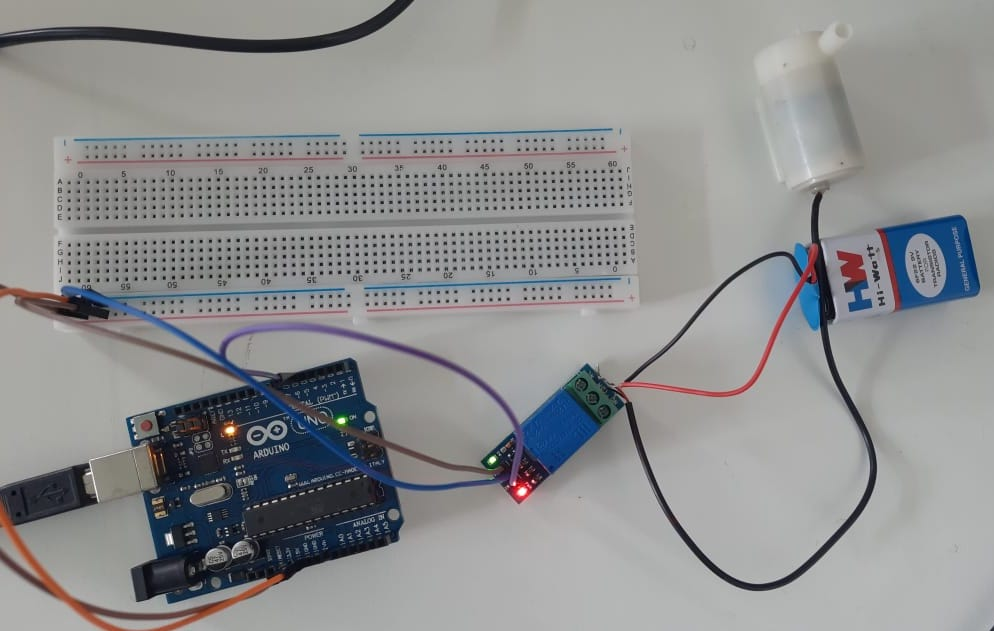
\includegraphics[scale=0.2]{relay-pump circuit.jpg}
    \caption{The relay-pump circuit}
    \label{fig:my_label}
\end{figure}

We set a lower limit (a minimum water level, 5cm below the ultrasound sensor) below which the pump would start functioning and filling water in the tub. How this worked was that the ultrasound sensor would give two consecutive readings of 5cm to the program, and that would give the relay a HIGH signal. The relay HIGH would switch the water pump on.

We also set an upper limit (a maximum water level, 4.25cm below the ultrasound sensor) above which the water pump would switch off and stop filling water. 

If an external signal was given to switch off the pump when the water was still below 4.25cm (we introduced a card between the water and the sensor between 4.25cm and 2cm from it), there are two cases:
\begin{itemize}
   
 \item Case 1: Water level is below 5cm: The moment you remove the external signal, the water pump would switch ON.

 \item Case 2: Water level is between 4.25cm and 5cm: The water pump would remain in the OFF state, because this water level is permissible according to our program.

\end{itemize}


\subsubsection*{The Arduino program for relay}
\begin{lstlisting}[style=Cstyle]


int controlInput=5;// output pin for sending signal from arduino to turn ON or OFF the pump

// here we used relay with NO- normally open mode, so when the controlInput is LOW, pump is ON and when the controlInput is HIGH, pump is OFF
void setup() {
  Serial.begin(9600);

  //configuring OUTPUT pin
  pinMode(controlInput,OUTPUT);

  //switch OFF the pump initially
  digitalWrite(controlInput,HIGH);
}

void loop() {
  // wait for 1 second
  delay(1000);
  //switch ON the pump for 3 second
  digitalWrite(controlInput,LOW);
  delay(3000);
  //switch OFF the pump 
  digitalWrite(controlInput,HIGH);
}
\end{lstlisting}

\subsection*{The final program}
\begin{lstlisting}[style=Cstyle]
int controlInput=5;
int trigger =4;
int echo=3;
long duration;
float distance;
int inputPin=2;
float flowRate;
// factor = pulses in 1 liter of water flow;
float factor=4330;
float volume;
float currentTime;
int counterStart=0,counterStop=0;
volatile unsigned long pulseCounter=0;
void setup() {
  Serial.begin(9600);
  pinMode(controlInput,OUTPUT);
  pinMode(inputPin,INPUT);
  digitalWrite(inputPin,HIGH);
  pinMode(trigger, OUTPUT);
  pinMode(echo,INPUT);
  digitalWrite(trigger,LOW);
  digitalWrite(controlInput,HIGH);
  attachInterrupt(digitalPinToInterrupt(inputPin),IRS_Counter,RISING);
  currentTime=millis();
  volume=0;
  counterStart=0;
  counterStop=0;
}

void loop() {
//  Serial.print("milis:");
//  Serial.println(millis());
  
  if(millis()-currentTime>=1000){
    detachInterrupt(digitalPinToInterrupt(inputPin));
    currentTime=millis();
    flowRate=(pulseCounter*60*1000)/factor;
    volume+=(flowRate/60);
      Serial.print("Pulse Count:");
      Serial.println(pulseCounter);
    Serial.print("Flow rate of water(in mL/min):");
    Serial.println(flowRate,DEC);
    Serial.print("Volume of water(mL):");
    Serial.println(volume,DEC);
      pulseCounter=0;
   attachInterrupt(digitalPinToInterrupt(inputPin),IRS_Counter,RISING);
    dist();
  }
 
}

void IRS_Counter(){
  pulseCounter++;
//  Serial.print("Pulse Count:");
//  Serial.println(pulseCounter);
}
void dist() {
  //delayMicroseconds(2);
  digitalWrite(trigger, HIGH);
  delayMicroseconds(10);
  digitalWrite(trigger,LOW);
  duration = pulseIn(echo,HIGH);
  distance=1.0*333*duration*100*(1e-6)/2;
  //print out the value of the pushbutton
  Serial.print("Duration:");
  Serial.println(duration);
  Serial.print("Distance(in cm):");
  Serial.println(distance);
  if(distance>5){
    counterStart++;
    if(counterStart>=3)
      digitalWrite(controlInput,LOW);
  }
  else{
    counterStart=0;
  }
  if(distance<=4.25)
  {
    counterStop++;
    if(counterStop>=2)
      digitalWrite(controlInput,HIGH);
  }
  else
  {
    counterStop=0;
  }
}
\end{lstlisting}

\begin{figure}[h!]
    \centering
    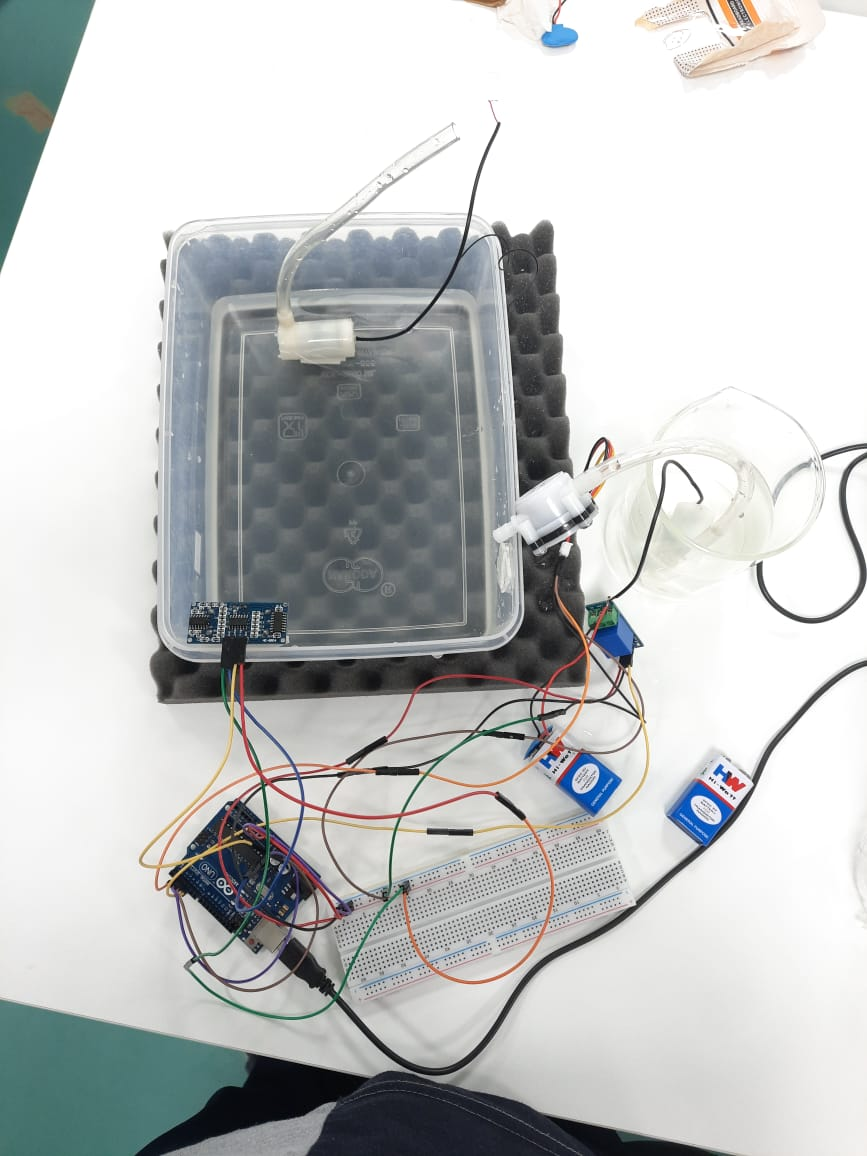
\includegraphics[scale=0.17, angle=90]{final circuit.jpg}
    \caption{The final circuit}
    \label{fig:my_label}
\end{figure}
\subsubsection*{Maintaining a fixed water level}

Some applications of this system require maintaining a fixed water level, so we made a few changes to the code to implement that. The only changes made here is removing the lower limit for the water level, and instead only keeping a counter for an upper limit (4.25cm here). Once the program gets three consecutive readings greater than 4.25, the pump will switch off, and any reading lower that than will switch the water pump on.

The counter was introduced to reduce faulty readings due to physical disturbances in the system.
\begin{lstlisting}[style=Cstyle]
void dist() {
  //delayMicroseconds(2);
  digitalWrite(trigger, HIGH);
  delayMicroseconds(10);
  digitalWrite(trigger,LOW);
  duration = pulseIn(echo,HIGH);
  distance=1.0*333*duration*100*(1e-6)/2;
  //print out the value of the pushbutton
  Serial.print("Duration:");
  Serial.println(duration);
  Serial.print("Distance(in cm):");
  Serial.println(distance);

  //maintain the level of water 4.25cm from sensor
  if(distance>4.25){
    counterStop=0;
    counterStart++;
    if(counterStart>=3)
      digitalWrite(controlInput,LOW);
  }
  else{
    counterStart=0;
    counterStop++;
    if(counterStop>=2)
      digitalWrite(controlInput,HIGH);
  
  }
}
\end{lstlisting}

Here's a link to a drive folder with more images and soft copies of our codes: \href{https://drive.google.com/drive/folders/1zCMMhSyvWyliZltZAFARa_KcmfMKBSfn?usp=sharing}{BM2003 Project}

\subsubsection*{References}
\href{https://www.epitran.it/ebayDrive/datasheet/YF-S401.pdf}{YF-S401 datasheet}\\
\href{https://cdn.sparkfun.com/datasheets/Sensors/Proximity/HCSR04.pdf}{HC-SR04 datasheet}

\begin{center}
   \textbf{The end.}
\end{center}


Project done by:

Samar Singhai   BM20BTECH11012\\
Vidya Ajay   BM20BTECH11017\\
Ramanathan Annamalai  BM20BTECH11011

\pagebreak
\end{document}
